\chapter{Extensive air shower parameters estimation}

\section{Shower photons discrimination}
\label{sec:signal-reconstruction}

During deconvolution, no assumptions are made about the presence or absence of an EAS photons in the signal. From optical detector simulation, we expect EAS photons to reach the mosaic in \textit{packets} --- groups of photons with an approximately normal arrival time distribution. Each packet can be described by three parameters: $n_{EAS}$ --- total number of photons in the packet, $\mu_t$ --- average photon arrival time, $\sigma_t$ --- standard deviation of arrival times. In the following, we define $\Theta \equiv (n_{EAS}, \mu_t, \sigma_t)$. The background (primarily, star and zodiacal light reflected from the snow) is modeled as Poisson-distributed photons with the average number $\lambda_{n}$ known from the calibration.

This problem can also be formulated as a Bayesian problem of finding a posterior distribution or EAS photons packet given the distribution of $\vec{n}$ obtained from the previous step (deconvolution).

First, let's consider a constant value of $\vec{n}$ and define the likelihood function for $\Theta$ in this case, i.e. the probability that the particular signal $\vec{n}$ was generated from the known background parameter $\lambda_{n}$ and an EAS packet with parameters $\Theta$. This can be easily done with the following Monte-Carlo: we sample a large number of photon arrival times following $\Theta$ ($n_{EAS}$ times $\sim \mathcal{N}(\mu_t, \sigma_t)$), convert each of them to histogram $\vec{n}_{\mathrm{signal}}$, calculate $\vec{n}_{\mathrm{background}} \equiv \vec{n} - \vec{n}_{\mathrm{signal}}$ and, finally, compute the probability that this set of background photon counts is a sample from Poisson distribution with mean $\lambda_{n}$ using the standard Poisson likelihood function.

\begin{equation}
	\mathcal{L}(\Theta) \equiv P(\vec{n} | n_{EAS}, \mu_t, \sigma_t) = \prod_{i} \frac{e^{-\lambda_n} \lambda_n^{n_{\mathrm{background}}^{(i)}}}{(n_{\mathrm{background}}^{(i)})!}
\end{equation}

Finally, to get the full likelihood function, given that $\vec{n}$ is defined by its posterior distribution, we have to average this exact likelihood over this distribution. Luckily, since we have not the posterior distribution itself, but a sample from it, we can just average the exact likelihood value over this sample.

Unlike the uninformative prior used for deconvolution, we can select meaningful priors $\Theta$ from Monte-Carlo simulation data: exponential distribution with $\lambda = 40$ for $n_{EAS}$, and $\mathcal{N}(2.4, 1)$ truncated at zero for $\sigma_t$. For $\mu_t$, a uniform prior over the signal frame was chosen.

After that, the same MCMC technique was used to get the final signal reconstruction result: posterior distribution of photon packet parameters $\Theta$. Performing both steps of the analysis within the same Bayesian framework lets us effectively chain these two analysis together, while also keeping them separate.

\subsection{Shower photon packet significance}

One of the advantages of a completely statistical approach is the ability to use the concept of significance to disciriminate the EAS and the background photons. We use Bayesian information criterion (BIC), introduced by Schwartz \cite{Schwarz1978} (in a sense, this is an Akaike's information criterion \cite{Akaike1974} adapted for Bayesian analysis). It states that several models describing data can be compared by the amount of information that is lost when replacing data with a model. The smaller the loss of information, the smaller the value of the criterion, and the better the model performs. The calculation is carried out according to the formula

\begin{equation}
	\mathrm{BIC} = k \ln n - 2 \ln \mathcal{L}_{max}
\end{equation}

Here $k$ is the number of model parameters, $n$ is the number of data sample elements, $\mathcal{L}_{max}$ is the maximum value of the likelihood function for the given model. As can be seen from the formula, BIC penalizes large number of parameters $k$.

To determine the significance of the found EAS signal, we compare two models: the <<background only>> model ($n_{EAS} = 0$) without parameters ($k=0$), and the <<background + signal>> model, described in the previous section, with $k=3$. The difference $ \Delta \mathrm{BIC} = \mathrm{BIC}_{noise} - \mathrm{BIC}_{background + EAS}$ shows the significance of the reconstructed signal. $\Delta \mathrm{BIC} \leq 0$ means the noise-only model is better, and such channels are considered empty. $0 < \Delta \mathrm{BIC} < 4$ means weak signal significance \cite{Kass1995}; in practice, we find that most deconvolution artifacts or strong background fluctuations fall into this region. Channels with $\Delta \mathrm{BIC} > 4$ are accepted as reliable (remaining false-positives are later eliminated during the shower geometry reconstruction). Figure \ref{pic:deconvolution-and-reconstruction} shows an example of full EAS photon packet parameters reconstruction for an experimental event.

\begin{figure}
	\centering
	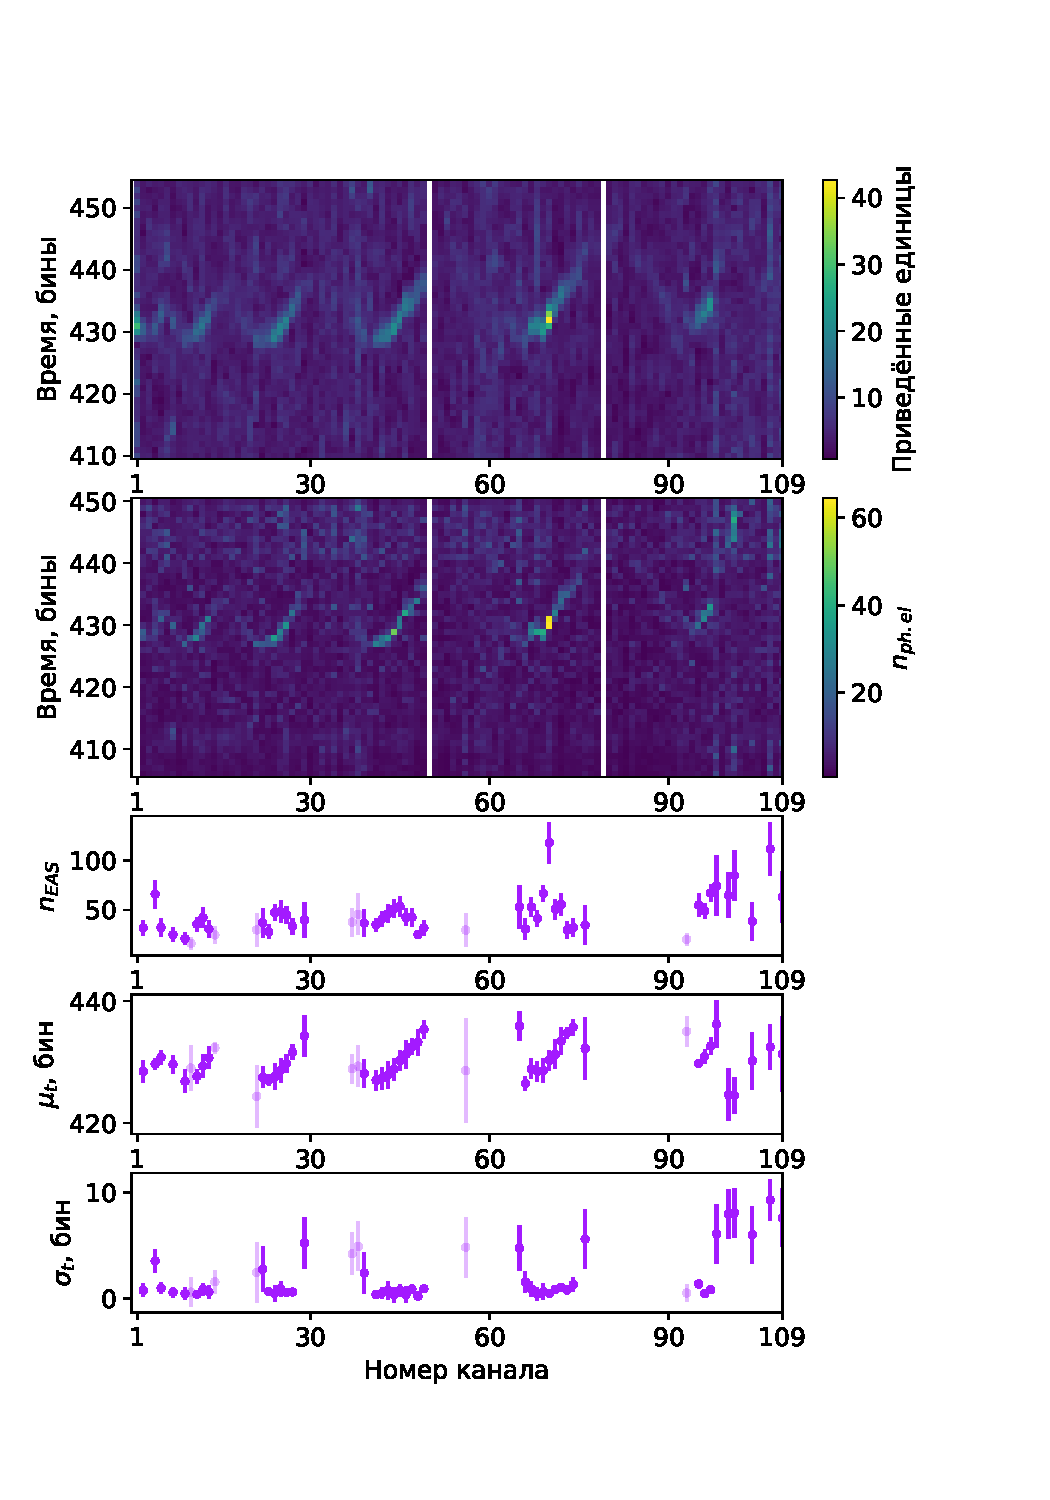
\includegraphics[width=0.86\columnwidth]{deconvolution-and-reconstruction}
	\caption{Full signal reconstruction for experimental event \#10675. Common X axis: channel number, see \cite{SphereCalibration2016} for numbering scheme. Top panel: experimental data with calibration coefficiens applied. Second-to-top panel: deconvolution output, photon count in each time bin. Three bottom panels: reconstructed photon packet parameters $n_{EAS}, \mu_t, \sigma_t$ --- dots and error bars represent marginal means and standard deviations; dimmed values are signals with $\Delta \mathrm{BIC} \in (0, 4]$, negative $\Delta \mathrm{BIC}$ (background-only channels) are omitted.}
	\label{pic:deconvolution-and-reconstruction}
\end{figure}


\section{Shower parameter reconstruction}

The rest of the reconstruction performed here in this work standard methods, with the exception of being applied to the output of Bayesian reconstruction.

\begin{itemize}
	\item \textbf{Shower arrival direction} is determined by a plain fit of arrival times. Ground level arrival times for each channel are determined from $\mu_t$ by subtracting ground-to-detector light travel time, accounting for the detector altitude and inclination.
	\item \textbf{Shower axis position} is determined by finding a point on the surface that maximizes the probability (with respect to each channel's posterior distribution) of monotonously decreasing lateral distribution function.
	\item \textbf{Lateral distribution function} for EAS Cherenkov light is determined by fitting a parametrized function to the data. In  this work, a simplified LDF from \cite{Budnev2005} is used. The fitting is done by convolving the LDF with each channel's light collection function (which is calculate from detector's optic system model). Shower energy is then derived from LDF parameters.
\end{itemize}
